\part{The Approach}

\section{The Conference}

\subsection{The Kind of Curiosity That Makes Money}

Michael Hart was in the audience.

Technically, he wasn’t supposed to be at the conference. A client meeting had fallen through, and instead 
of flying out early, he decided to walk the floor. Kill a day. Stay curious. The kind of curiosity 
that made money.

The conference center was all beige carpet, branded lanyards, and tepid coffee in compostable cups. Rows of 
LED-lit booths advertised “responsible AI,” “quantified resilience,” and “next-gen compliance intelligence.” 
One corner featured a sponsored espresso bar. Another had massage chairs under a banner that read: 
\textit{“De-risk your week.”}

Hart didn’t blend in. Not just because of the Tom Ford suit or the black-on-black oxford shoes. It was the 
way he moved: not networking, but hunting. While others nodded through panels with the slack-jawed politeness 
of jetlagged consultants, Hart listened.

Really listened.

He sat two rows from the front. Elbows on knees. Eyes narrowed slightly. And by the second case study, he knew.

This wasn’t just another founder spinning buzzwords. David had edge. The kind that didn’t come from pitch decks. 
The kind that came from bloodied prototypes and quiet bets placed at 2 a.m.

After the panel, while others queued for coffee or badge scans, Hart moved straight toward the stage. No small talk. 
No handshake.

“I’ve got distribution,” he said. “You’ve got product.”

He handed David a white and unembossed business card with just a name, number, and a discreet logo in matte black.

“Let’s talk.”

Then he walked away with the kind of exit that didn’t invite follow-up.

Hart was the founder of Centauri Consulting, which billed itself as “the velvet glove of high-stakes transformation.” 
He didn’t just sell strategic roadmaps. He sold access. His firm specialized in landing contracts other firms 
couldn’t even bid for: the kind where success wasn’t measured in deliverables, but in who picked up the phone.

Centauri didn’t advertise. It didn’t recruit on LinkedIn. It wasn’t looking for clients.

It was looking for \textbf{technical talent it couldn’t poach outright}.


\medskip

\begin{HistoricalSidebar}{The Dark Side of Acquihires --- When Talent Becomes Leverage}

  In the early 2000s, as Silicon Valley’s war for engineering talent reached fever pitch, a new acquisition model 
  quietly took over the startup ecosystem: the \textbf{acquihire}.

  \medskip
  
  Unlike a traditional acquisition, where the buyer wants the product, patents, or market share, an acquihire’s primary 
  target is \textbf{the team}. The startup itself might be shut down, its technology shelved, its users abandoned. The 
  engineers were the real asset.

  \medskip
  
  At first, acquihires were framed as \textit{soft landings} for struggling startups—a face-saving way to pay back 
  investors, a lifeboat for founders, a pathway into Big Tech.

  \medskip
  
  But beneath the glossy press releases, a harsher reality unfolded.

  \medskip
  
  Founders often found themselves negotiating from a position of desperation, their options underwater, their runway gone. 
  Investors pressured them to “return something” rather than risk a total wipeout. Engineers were given golden handcuffs: 
  lucrative retention bonuses tied to multi-year employment agreements, conditional on project milestones that conveniently 
  reset their vesting clocks.

  \medskip
  
  In some cases, acquihires functioned as \textbf{talent raids disguised as mergers}. A competitor could eliminate a rival’s 
  core team while burying its roadmap. A corporation could sidestep a hiring freeze by acquiring headcount off the books.

  \medskip
  
  And for founders, the acquihire wasn’t always an exit—it was a quiet exile.
  
  \medskip
  
  The deeper lesson?

  \medskip
  
  An acquihire doesn’t just buy talent. It \textbf{absorbs leverage}. It converts independent actors into vested stakeholders, 
  ties reputations to institutional outcomes, and rewrites incentives through retention clauses and non-compete agreements.
  Because The real deal isn’t written in the press release.  The real deal is written in the clauses that keep you from leaving.
  
\end{HistoricalSidebar}


\subsection*{Editor Questions for ``The Kind of Curiosity That Makes Money''}

This scene introduces a new power player and reframes the protagonist through someone else’s lens. It’s a moment of recognition — and recruitment. The questions below are meant to help interrogate how that shift lands, both in terms of character development and larger thematic arcs. Focus on what sparked interest, what felt flat, and how this changes your view of the story’s stakes.

\subsubsection{Narrative \& Structure}

\begin{itemize}
  \item Did the scene feel like a natural progression from what came before? Or did it feel like a tonal shift?
  \item Was the pacing effective — particularly the transition from exposition to Hart’s proposition?
  \item Did the sidebar feel integrated or interruptive in this section? Did it add context or dilute the main thread?
\end{itemize}

\subsubsection{Emotional \& Psychological Resonance}

\begin{itemize}
  \item How did Hart’s entrance change the emotional temperature of the story?
  \item Did his approach to David (direct, transactional, predatory) feel thrilling, unsettling, or something else?
  \item What emotion lingered most after reading this section: excitement, unease, tension, admiration?
\end{itemize}

\subsubsection{Character Insight}

\begin{itemize}
  \item What did this scene reveal about Hart? About David?
  \item Did Hart feel like a real person or an archetype? Did that help or hinder the scene?
  \item Based on this interaction, what kind of relationship do you expect between Hart and David? Mutually beneficial? Manipulative? Symbiotic?
\end{itemize}

\subsubsection{Thematic Depth}

\begin{itemize}
  \item What larger themes does this scene activate? Power? Ambition? Exploitation? Institutional seduction?
  \item Did the acquihire sidebar enrich your understanding of the stakes — or pull focus away?
  \item Was the metaphor of “absorption of leverage” compelling? Did it feel like an exaggeration, or did it resonate?
\end{itemize}

\subsubsection{Style \& Craft}

\begin{itemize}
  \item Was there a specific line or image that stuck with you? (e.g., “the kind of curiosity that makes money,” “vested stakeholders,” etc.)
  \item Did the scene’s description (setting, tone, dialogue) help you visualize the world? Or did it feel overly abstract?
  \item Did the transition from conference-floor banality to backroom intensity work for you?
\end{itemize}

\subsubsection{Deeper Testing}

\begin{itemize}
  \item What would be lost if this scene were cut? What would be gained?
  \item How would your perception of David’s arc shift if this interaction with Hart happened later — or earlier?
  \item If this were the first scene you read, what genre or narrative stakes would you expect from the story?
\end{itemize}



\section{The Conversation}

\subsection{The Pitch Behind the Pitch}

They met in the quiet lounge just off the mezzanine with
velvet chairs, filtered light, and a silent espresso machine in the corner that looked sculptural but hissed like a 
snake when used. 

Hart didn’t waste time.

``I’ve seen pitch decks with less clarity than your case study,'' he said with settling into the chair opposite David 
without removing his coat.

David nodded, cautiously. The coffee in his hand was mostly cold. He wasn’t used to being approached like this.

``You built that yourself?'' Hart asked.

``Yeah,'' David said. ``Most of it.''

``What’s your background?''

``Quant. I used to build pricing models at a high-frequency shop.'' 
He hesitated. ``We blew up during the COVID carry unwind. No fraud. Just... leverage and luck.''

Hart raised an eyebrow. ``So instead of finding another job, you decided to build one.''

David half-smiled. ``Something like that.''

He explained the idea: a compliance tool --- built with the precision of trading infrastructure --- that could 
automate the data due diligence financial regulators required.  
Not just a checklist. A framework. Something that could scan model documentation, track revision histories, flag 
missing disclosures, and render it all into audit-grade reports.

Hart sat forward. His gaze sharpened.

``You’re not building regtech,'' he said. ``You’re building capacity.''

David looked puzzled.

Hart clarified: ``You’re not replacing a process. You’re replacing a personnel problem.''

He laid it out plainly. 

Most mid-tier hedge funds were boxed in. They didn’t have the budget to hire elite ML compliance engineers. 
Or, that talent went straight to Goldman, Citadel, or was padded behind big-tech RSUs. 
The rest are hard to find, and even harder to keep.

``If you can get those shops to 80\% compliant without hiring a team to maintain the stack,'' Hart said, ``you’re not 
just solving a problem. You’re leveling the field.''

David said nothing. The hum of the nearby HVAC unit filled the pause.

Hart didn’t mind the silence. He leaned back just slightly, as if to signal: you’re the one being interviewed now.

``You won’t make them Goldman,'' he said. ``But you’ll lower the barrier to entry. That’s enough. That’s how markets shift.''

Then, softer, more pointed:

``You don’t need my validation. You’ve got product. What you need is volume.''

He tapped the card he’d laid on the table.

``I know who needs this. Let’s talk.''

\medskip

\begin{HistoricalSidebar}{The Anatomy of a Value Proposition: Why Some Products Land and Others Stall}

  A \textbf{value proposition} is not what a product \textit{does}. It's what it \textbf{solves}. And in markets 
  crowded with technical talent and noise, clarity about that distinction can determine whether a startup takes 
  off or disappears.
  
  \medskip
  
  In startup mythology, product-market fit often gets all the attention. But what gets overlooked is \textbf{problem-founder fit}: 
  whether the founder truly understands the pain they’re solving — and who has it.
  
  \medskip
  
  \textbf{Successful Example: Stripe (2010)}  
  Most payment platforms in 2010 focused on buyers. Stripe targeted \textit{developers} — the engineers tasked with integrating 
  payment APIs. Their value proposition wasn’t “payments made easy,” it was:  
  \textit{“You can deploy a full payments stack in 7 lines of code.”}  
  The problem wasn’t payments — it was \textbf{friction}. Stripe solved for the person who had to ship working code by the end 
  of the week.
  
  \medskip
  
  \textbf{Failed Example: Color Labs (2011)}  
  Color Labs raised \$41 million to launch a social photo app that let users share images with people nearby. The technology 
  was novel — using GPS and proximity to build social networks on the fly — but the value proposition was fuzzy:  
  \textit{“Take pictures together in real-time.”}  
  What problem did it solve? Who needed it? Why now? Users didn’t know. Neither did investors by the time it folded.
  
  \medskip
  
  \textbf{Gray Zone Example: Juicero (2013)}  
  Juicero’s product — a \$400 cold-press juicer — was marketed as a health-tech device with subscription-based juice packets. 
  On paper, it sounded modern and slick. But once people realized you could squeeze the packets by hand, the core value 
  proposition evaporated:  
  \textit{It wasn't about juice. It was about perceived luxury.}  
  The mismatch between actual utility and projected status killed the brand.
  
  \medskip
  
  \textbf{The lesson?}  
  Value proposition design isn’t about feature lists — it’s about mapping your product to a very specific bottleneck in someone 
  else’s world. The sharper the bottleneck, the clearer the value.
  
  \medskip
  
  That’s why Hart zeroed in on David’s tool. Not because it was novel, but because it solved a specific institutional constraint:  
  “Get to 80\% compliance without hiring.”
  
\end{HistoricalSidebar}

\subsection{Flattening the Curve}


The second pour of scotch had softened the edges.

They were seated in the lounge of the downtown private club — all brushed brass and low lighting, the kind of place 
designed to look expensive without feeling new. Outside, the city buzzed with Thursday night urgency, but inside, 
everything moved slower. Intentional. The table was marble, veined with gold, chilled to the touch. The waiter had 
long since faded into the background.

The pitch was over. Now came the calculus.

Hart leaned in, elbows on the stone.

“You’re not building a compliance product,” he said. “You’re building a keycard.”

David blinked once, slowly. “Keycard?”

Hart didn’t smile. He clarified without condescension:

“You’re not solving for oversight. You’re solving for access. You’re handing mid-tier funds a way into a market they were 
never allowed to touch.”

On the other side of the table, Penn looked up from the term sheet he’d been annotating with a silver Montblanc. He didn’t 
interrupt. Just listened.

Hart continued:

“High-frequency trading isn’t locked off because of regulation. It’s locked off because of stack complexity. 
Infrastructure. Latency. State handling. Data streaming. And yeah, regulatory overlays, but those come after.”

David nodded slowly, his fingers wrapped around the base of his glass. “Most of them don’t even try. The bar’s too high.”

“Exactly,” Hart said. “They’re priced out by the engineering curve. Not the compliance curve. You flatten that curve, you 
open the gate.”

The ice in David’s glass cracked gently, like it had been waiting for the moment.


\medskip

\begin{TechnicalSidebar}{Barriers to Entry and Why Most Funds Stay Out}

  A \textbf{barrier to entry} is anything that prevents a new player from entering a market and competing effectively.  
  These barriers aren’t always regulatory. In fintech and high-frequency trading (HFT), they’re often 
  \textit{technical, infrastructural, or cultural}.
  
  \medskip
  
  \textbf{In HFT and ML-driven trading, the primary barriers include:}

  \medskip
  
  \begin{itemize}
    \item \textbf{Stack Complexity:}  
    Millisecond-level latency requirements, real-time introspection, and fault-tolerant event handling pipelines.
  
    \item \textbf{Talent Scarcity:}  
    Engineers who understand trading systems, compliance hooks, and low-level performance tuning are rare — and expensive.
  
    \item \textbf{Regulatory Overlay:}  
    Once infrastructure exists, it must also meet legal standards — audit logs, fair execution, capital disclosures — without slowing performance.
  
    \item \textbf{Reputational Signaling:}  
    Even with a working stack, institutional allocators are wary of unknown platforms without validation from top-tier logos.
  \end{itemize}
  
  \medskip
  
  \textbf{The Result?}  
  Even well-capitalized funds avoid building from scratch.  
  Not because they don’t want to — but because the path to parity is too steep, too slow, and too expensive.
  
  \medskip
  
  \textbf{The strategic unlock?}  
  Build a system that \textit{collapses the engineering barrier} without compromising regulatory posture.  
  Suddenly, you’re not selling software. You’re selling \textbf{access}.
  
\end{TechnicalSidebar}


\medskip

The scotch had mellowed, but the air stayed sharp from the clarity that only comes when no one’s 
pretending anymore. The room had the lacquered hush of old money: recessed lights, no music, and walls lined with abstract 
art chosen more for tax deduction than taste.

Outside, the city blurred under halogen and mist, but in here, everything had slowed to a crisp, analytical tempo.

David described the pipeline again as a vertical-integration play:  
an internal model engine, backtesting under stress scenarios, pipeline introspection, and compliance hooks all rendered 
into modular, containerized deploys.

“You don’t build a product,” Hart said. “You build entry velocity.”

David raised an eyebrow. “Meaning?”

Hart smiled faintly, resting his glass on the marble.

“Meaning they can go from zero to trading without hiring Citadel’s shadow stack.”

Penn folded the term sheet and tapped the cover with two fingers, like sealing an envelope.

“So you’re not selling features. You’re selling qualification.”

“Exactly,” Hart replied. “Most people fail the entry exam. You let them cheat.”

Hart pivoted, now sketching the business model in the air with his hand.

“You don’t price it like a SaaS tool. You price it like a futures contract.  
You’re not charging for usage. You’re charging for entry rights.”

David stayed silent. This wasn’t how he had framed it, but it clicked.  
Not a toolkit. Not a reg layer.

A gateway.

And gateways? Those get priced by what they unlock.



\subsection{Napkin Math and Synthetic Margins}

The bar was dim, upscale but unpretentious. It was the kind of place where the lighting was low enough to suggest intimacy, 
but not so low that you couldn’t read a term sheet. A jazz trio murmured in the corner, and the leather booths smelled 
faintly of cedar and citrus polish.

Hart pulled a cocktail napkin toward him and clicked a pen from his jacket. He didn’t bother asking for a fresh sheet of paper.

``Let’s run the numbers,'' he said, scribbling a row of assumptions down the margin. ``Not investor math. 
Fermi math.''

Morales grinned and leaned in. ``Back-of-the-envelope?''

``Always,'' Hart said. ``It’s not about precision. It’s about order of magnitude sanity.''

He drew three columns: headcount, compliance burden, deployment velocity.

``Say a fund with \$300 million AUM wants to scale into synthetic credit. Normally they’d need --- what? --- five 
headcount just to maintain reporting compliance?''

\medskip

\begin{TechnicalSidebar}{What is Synthetic Credit?}

  \textbf{Synthetic credit} refers to exposure to credit risk through financial derivatives—rather than through direct 
  ownership of bonds or loans.

  \medskip
  
  Unlike traditional credit instruments (e.g., corporate bonds), synthetic credit positions are created using tools 
  such as:

  \medskip
  
  \begin{itemize}
    \item \textbf{Credit Default Swaps (CDS):}  
    A CDS functions like credit insurance. The buyer pays a regular premium to the seller, and in return, gets 
    compensated if a third-party borrower (like a company or government) defaults.  

    \medskip
  
    \textit{Example:} It's like paying monthly insurance on a neighbor’s mortgage. However, you don’t own the house, but 
    you’ll get a payout if they default on the loan.


    \medskip
  
    \item \textbf{Total Return Swaps (TRS):}  
    In a TRS, one party agrees to hand over the total return (interest + price appreciation) from a credit asset 
    in exchange for a fixed or floating payment.  

    \medskip
  

    \textit{Example:} Imagine you own a risky bond, but instead of collecting its unpredictable income, you trade 
    it for steady monthly rent and give someone else the upside (and risk) in exchange for certainty.


    \medskip
  
    \item \textbf{Structured Notes or Options:}  
    These are custom-built financial products based on baskets of credit indices or portfolios, often with embedded 
    features like leverage or downside protection.  

    \medskip
  

    \textit{Example:} Think of it like a chef's tasting menu. You're not just betting on one credit, but on a handpicked 
    combo of bonds or indices, with special ingredients like caps, floors, or trigger conditions that shape how 
    (and if) you get paid.
  \end{itemize}

  \medskip
  
  These instruments allow funds to scale exposure rapidly without purchasing underlying assets. They're cheaper, faster, 
  and more capital-efficient, but also more opaque.

  \medskip

  \begin{figure}[H]
    \centering
    \resizebox{0.92\textwidth}{!}{%
      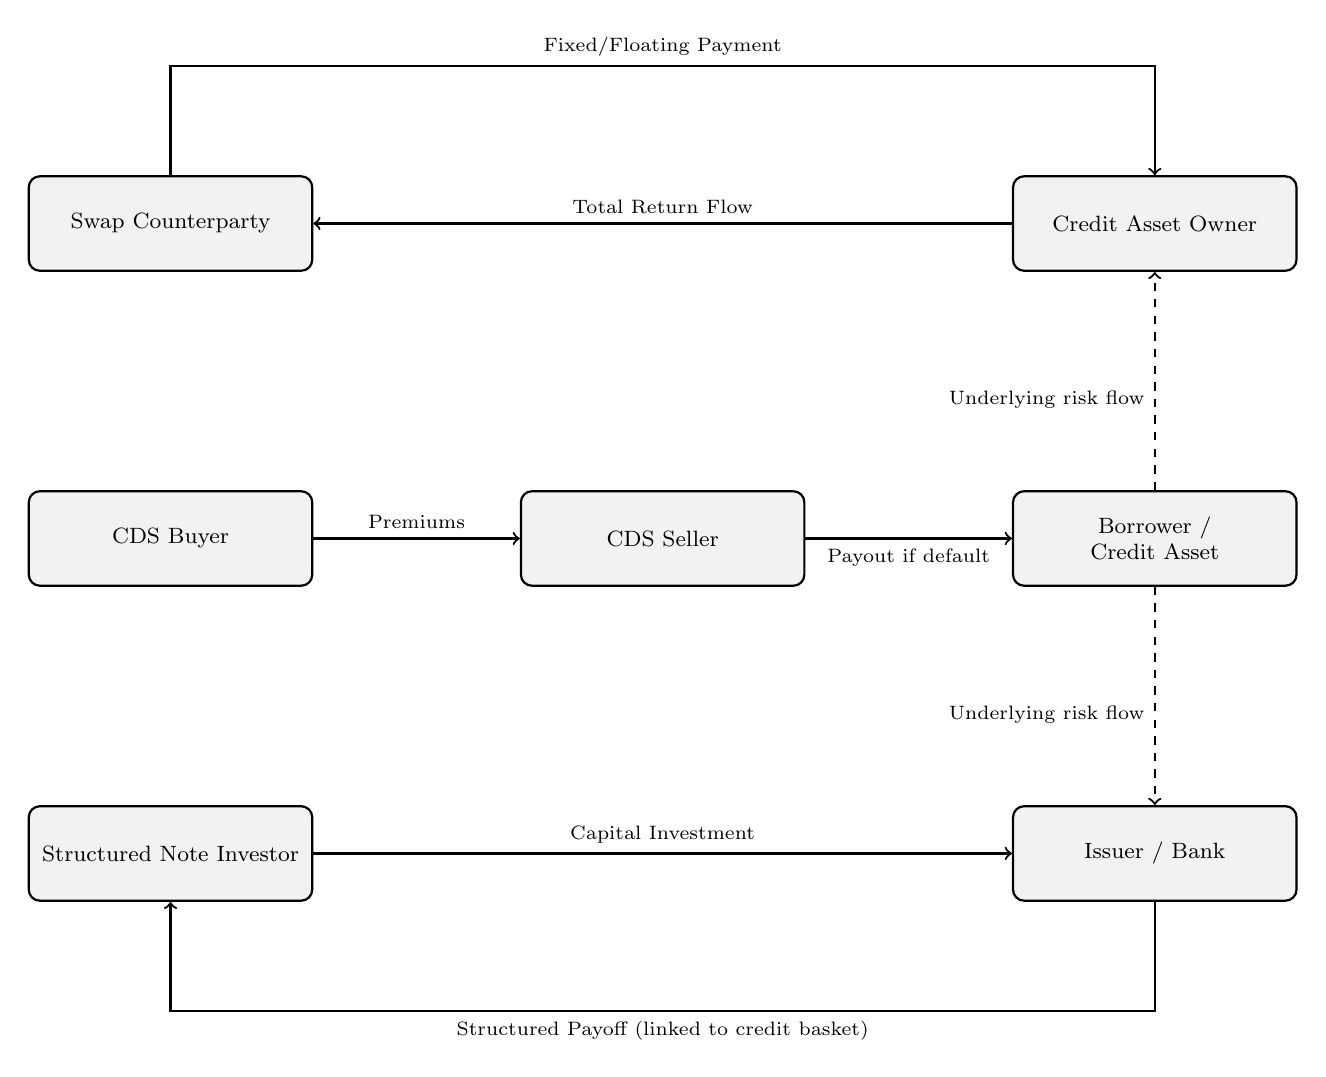
\begin{tikzpicture}[
        font=\footnotesize,
        box/.style={draw, thick, rounded corners, minimum width=3.6cm, minimum height=1.2cm, align=center, fill=gray!10},
        arrow/.style={->, thick},
        note/.style={font=\scriptsize\itshape},
        x=2.5cm, y=2cm
      ]
  
      % Source of risk
      \node[box] (borrower) at (5,0) {Borrower /\\Credit Asset};
  
      % CDS
      \node[box] (cdsbuyer) at (0,0) {CDS Buyer};
      \node[box] (cdsseller) at (2.5,0) {CDS Seller};
  
      \draw[arrow] (cdsbuyer) -- node[above] {\scriptsize Premiums} (cdsseller);
      \draw[arrow] (cdsseller) -- node[below] {\scriptsize Payout if default} (borrower);
  
  
      % TRS
      \node[box] (trsasset) at (5,2) {Credit Asset Owner};
      \node[box] (trsparty) at (0,2) {Swap Counterparty};
  
      \draw[arrow] (trsasset) -- node[above] {\scriptsize Total Return Flow} (trsparty);
      \draw[arrow] (trsparty) 
        -- ++(0, 1) coordinate (drop)
        -- ++(+2.5, 0) coordinate (midpoint)
        -|
        (trsasset);

      \node[above] at (midpoint) {\scriptsize Fixed/Floating Payment} (trsasset);
  
  
      % Structured Notes
      \node[box] (investor) at (0,-2) {Structured Note Investor};
      \node[box] (issuer) at (5,-2) {Issuer / Bank};
  
      \draw[arrow] (investor) -- node[above] {\scriptsize Capital Investment} (issuer);
      \draw[arrow] (issuer) 
        -- ++(0, -1) coordinate (drop)
        -- ++(-2.5, 0) coordinate (midpoint)
        -|
        (investor);
      \node[below] at (midpoint) {\scriptsize Structured Payoff (linked to credit basket)};


  
  
      % Borrower arrow
      \draw[arrow, dashed] (borrower) -- node[below left] {\scriptsize Underlying risk flow} (trsasset);
      \draw[arrow, dashed] (borrower) -- node[below left] {\scriptsize Underlying risk flow} (issuer);

      %\node[note] at (-2,2.6) {CDS shifts default risk};
      %\node[note] at (4,0.8) {TRS swaps performance for certainty};
      %\node[note] at (2.5,-3.3) {Notes repackage risk into custom products};
  
      \end{tikzpicture}%
    }
    \caption{How Credit Derivatives Distribute or Transform Credit Risk}
  \end{figure}

  \medskip
  
  \textbf{Why use it?}  

  \medskip

  Funds deploy synthetic credit to:

  \medskip
  
  \begin{itemize}
    \item Express directional credit views without taking balance sheet risk
    \item Hedge credit portfolios with speed and precision
    \item Amplify leverage in a regulatory-compliant wrapper
  \end{itemize}

  \medskip
  
  \textbf{The tradeoff:}  
  
  \medskip

  While synthetic credit boosts flexibility and velocity, it can distort actual exposure metrics. During stress events, 
  the correlation between synthetic and physical markets can break down—causing ``drift'' between expected protection 
  and realized loss.

  \medskip
  
  This divergence played a central role in multiple financial dislocations, including the 2008 collapse of AIG’s CDS 
  book, and more recently, in smaller liquidity ruptures triggered by undercapitalized synthetic tranches.
  
\end{TechnicalSidebar}

\medskip

``Minimum,'' David said. ``Assuming no turnover.''

``Right,'' Hart said, underlining the number. ``Now suppose your pipeline replaces three of those roles 
and reduces latency by 60\%. What does that buy them?''

``Speed to market. And internal optics.''

Hart nodded. ``And optics translate into allocation. Faster compliance means faster scaling.''

He tapped the napkin, now smudged with numbers and ink streaks.

``That’s your margin,'' he said. ``Not in features. In time arbitrage.''

David stared at the scribbled napkin. The math was loose. But the logic was airtight.

He didn’t need a calculator. He needed a clock.

And Hart had just reset it.

\medskip


\begin{HistoricalSidebar}{Fermi Estimation: How Atomic Physics Became a Quant Interview Question}

  In July 1945, at the Trinity nuclear test site in New Mexico, Enrico Fermi stood among a group of physicists waiting for 
  history to unfold.  
  As the countdown to the first atomic explosion reached zero, Fermi performed an odd, almost casual act: he dropped small 
  scraps of paper.
  
  \medskip
  
  When the shockwave from the detonation reached him, he observed how far the papers had traveled.  
  From that simple displacement, he estimated the blast yield at approximately 10 kilotons of TNT.
  
  \medskip
  
  Official measurements later put it at about 18.6 kilotons — meaning Fermi, with no instruments and only a handful of confetti, 
  was within a factor of 2.
  
  \medskip
  
  This moment became legend: not because of the accuracy, but because of the method.  
  Fermi didn’t measure. He decomposed the problem into approximate parts — what we now call a \textbf{Fermi estimate}.
  
  \medskip
  
  \textbf{Fermi estimation} is a mental technique for approximating a quantity using only logical reasoning and 
  order-of-magnitude assumptions.  
  It’s the art of going from ``I have no idea'' to ``I have a rough sense'' using structured guesswork.
  
  \medskip
  
  \textbf{The canonical example:}  
  How many piano tuners are there in Chicago?

  \medskip
  
  \begin{itemize}
    \item Population of Chicago: \textasciitilde3 million  
    \item Average household size: 2.5 $\Rightarrow$ 1.2 million households  
    \item Households with pianos: \textasciitilde1 in 20 $\Rightarrow$ 60,000 pianos  
    \item Tunings per piano per year: 1  
    \item Total tunings: 60,000/year  
    \item A tuner can do 4 jobs/day, 5 days/week, 50 weeks/year = 1,000 tunings/year  
    \item Needed tuners: 60,000 / 1,000 = \textbf{60 piano tuners}
  \end{itemize}
  
  \medskip
  
  Of course, the real number might be 50 or 80. But that’s not the point.  
  What matters is the \textbf{reasoning}.
  
  \medskip
  
  That’s why Fermi questions became a staple of quant interviews, startup pitches, and market strategy sessions.  
  They don’t test precision.  
  They test \textbf{decomposition, intuition, and the courage to guess}.
  
  \begin{quote}
  \textit{“All models are wrong,”} the saying goes, \textit{“but some are useful.”}  
  Fermi estimates live in that exact margin.
  \end{quote}
  
  \medskip
  
  Whether estimating nuclear yields or billion-dollar TAMs, Fermi logic reminds us:  
  You don’t need perfect data to make a high-quality decision.  
  You just need the guts to bound the problem — and the clarity to own your assumptions.
  
\end{HistoricalSidebar}
  

\subsection{A Market Just Deep Enough}

The napkin was already cluttered, but Hart kept writing.

``There are about 5{,}000 hedge funds globally,'' he said, thinking aloud. ``Call it 2{,}000 
that are small-to-mid tier. The kind that can’t build their own infra stack.''

David leaned over the table.

``Assume 5\% are actively trying to expand into ML-based quant. That’s 100 funds.  
We could reasonably sell to half over five years if we build a reputation. So 50 logos?''

Hart nodded.

``Call it 10 the first year. If they pay \$250{,}000 each, that’s \$2.5 million topline.  
Think pilot licenses, integration, and support.''

David sipped his drink. ``And that’s before we license the IP or run API-based usage tiers.''

``Exactly,'' Hart said. ``If even 20\% of the target market scales usage and upgrades to \$500{,}000 per year,  
we’re looking at \$10–15 million annual run rate within 3 years.''

David tapped the napkin.

``So you frame it like this:''

The napkin was a mess — arrows, margins crowded with dollar signs, numbers scribbled into a funnel. But as David 
stared at it, something clicked.

It reminded him of how he got his first job.

Not from a polished resume — but from answering a market sizing question scrawled on the back of a flyer at a campus event.
“Size the market for enterprise AI in logistics.” No internet. No prep.

He broke it down on the spot — industry size, adoption curve, price points — drew a funnel, gave a number.
Rough. Fast. Believable.

That got him in the door.

Now here he was, years later, doing the same thing —
2,000 funds → 5\% early adopters → 50 clients → \$250k each.

No slides. Just ink and instinct.

And for a moment, he smiled.
The math hadn’t changed.
Only the stakes had.

\medskip

\begin{figure}[H]
    \centering
    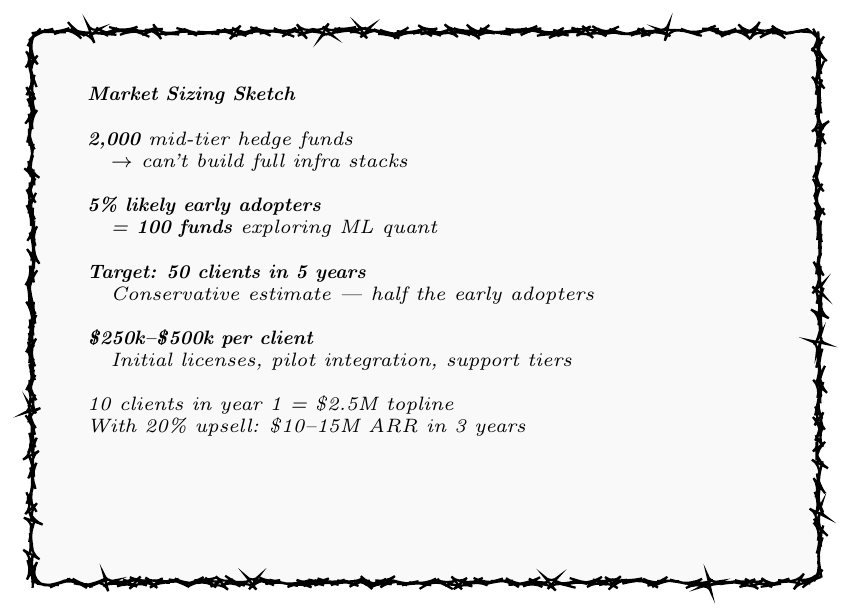
\begin{tikzpicture}[
      font=\footnotesize,
      fuzz/.style={draw=black, thick, rounded corners, fill=gray!5, decorate, decoration={random steps, segment length=2pt, amplitude=1pt}},
      txt/.style={align=left, font=\scriptsize\itshape},
    ]
  
    % Napkin box
    \node[fuzz, minimum width=10cm, minimum height=7cm, anchor=north west] (napkin) at (0,0) {};
  
    % Content inside
    \node[txt, anchor=north west] at ([xshift=0.6cm, yshift=-0.6cm]napkin.north west) {
      \textbf{Market Sizing Sketch} \\
      \\
      \textbf{2{,}000} mid-tier hedge funds \\
      \quad $\rightarrow$ can't build full infra stacks \\
      \\
      \textbf{5\% likely early adopters} \\
      \quad = \textbf{100 funds} exploring ML quant \\
      \\
      \textbf{Target: 50 clients in 5 years} \\
      \quad Conservative estimate — half the early adopters \\
      \\
      \textbf{\$250k–\$500k per client} \\
      \quad Initial licenses, pilot integration, support tiers \\
      \\
      \textit{10 clients in year 1 = \$2.5M topline} \\
      \textit{With 20\% upsell: \$10–15M ARR in 3 years}
    };
  
    \end{tikzpicture}
    \caption{Napkin Summary: Market sizing and revenue projection for ML quant infrastructure sales.}
\end{figure}

\medskip

Hart leaned back, smiling.

``Exactly. Market isn’t huge. But it’s deep. It's high trust, high margin, and high retention.  
And once the first five logos land, the rest follow.  
Because nobody wants to be the last quant fund without a real-time audit layer.''

David nodded slowly.

``And if you wrap the IP into a licensing structure, the revenue multiple goes from 5x to 12x overnight.  
TAM is maybe \$500 million globally. We don’t need it all. We just need the perception that we could take 10\%.''

Hart smirked.

``And that’s how you Fermi your way into a \$50 million valuation in the first year after deployment.''


\medskip

\begin{TechnicalSidebar}{Business Viability, Payback Period, and Why VCs Care About Speed}

  One of the most underrated metrics in early-stage venture capital isn’t TAM, burn rate, or even ARR.  
  It’s \textbf{payback period} — the time it takes for a new customer to generate enough revenue to cover their own acquisition cost.
  
  \medskip
  
  \textbf{Payback Period Formula:}
  \[
  \text{Payback Period} = \frac{\text{Customer Acquisition Cost (CAC)}}{\text{Gross Margin from Customer per Month}}
  \]
  
  \medskip
  
  If it costs \$50,000 to close a deal and that customer brings in \$25,000 per month in margin,  
  the payback period is 2 months.
  
  \medskip
  
  \textbf{Why it matters:}
  
  \begin{itemize}
    \item Short payback = fast reinvestment cycles. A startup can recycle revenue into more growth without needing new funding.
    \item Long payback = higher risk. The startup must float costs for months (or years) before breakeven.
    \item For VC firms, short payback implies \textbf{capital efficiency} — every dollar deployed drives quicker returns.
  \end{itemize}
  
  \medskip
  
  In the case of Hart and Morales’ strategy:

  \medskip
  
  \begin{itemize}
    \item Each client pays \$250K to \$500K annually.
    \item The product is deployed quickly — modular, containerized, low-integration overhead.
    \item Gross margins exceed 80\%, given the IP-heavy, low-support model.
  \end{itemize}
  
  \medskip
  
  Even assuming \$50K to acquire each customer, they break even within 3 months.  
  That puts them in elite territory — where CAC is recouped before the second quarter, and LTV/CAC ratios can exceed 8x.
  
  \medskip
  
  \textbf{The VC view:}  
  This isn’t just a niche tool. It’s a high-trust, high-ticket product with low churn and fast returns.
  
  \begin{quote}
  \textit{In venture math, velocity beats volume.  
  A product that pays itself back in 90 days can be scaled   
  (even before it's perfect).}
  \end{quote}
  
\end{TechnicalSidebar}
  

\medskip

\subsection{Narrative as a Moat}


Hart was drawing boxes on the napkin again.

``Let’s scale this. Think beyond hedge funds. Who else needs this?''

David didn’t hesitate.  
``Anyone algorithmically allocating capital under regulatory pressure:
  Banks with quant desks;  
  Sovereign wealth arms; 
  Insurance and pensions migrating into automated trading; 
  Even crypto funds trying to look institution-grade''

Hart tapped his pen twice. ``So what’s the real market size?''

David ran the numbers aloud.

``Globally? Maybe 30{,}000 institutional allocators.  
Say 10{,}000 are actively integrating ML or automation over the next five years.  
Conservatively, 20\% are in position to buy infra — that’s 2{,}000 serious prospects.''

Hart grinned. ``Then we blitz it.''

David raised an eyebrow. ``You’re saying go wide before we even optimize?''

``Exactly,'' Hart replied. ``Control’s a second-mover problem.  
Right now, we’re building surface area. \$500K/year base. \$1 million-plus for full access: audit layer, 
traceability, and IP hooks.  
You don’t trickle this in. You carpet-bomb the category. Own the narrative before anyone else knows 
there’s a war.''

David scratched numbers into the corner of the napkin.

\medskip

\begin{figure}[H]
    \centering
    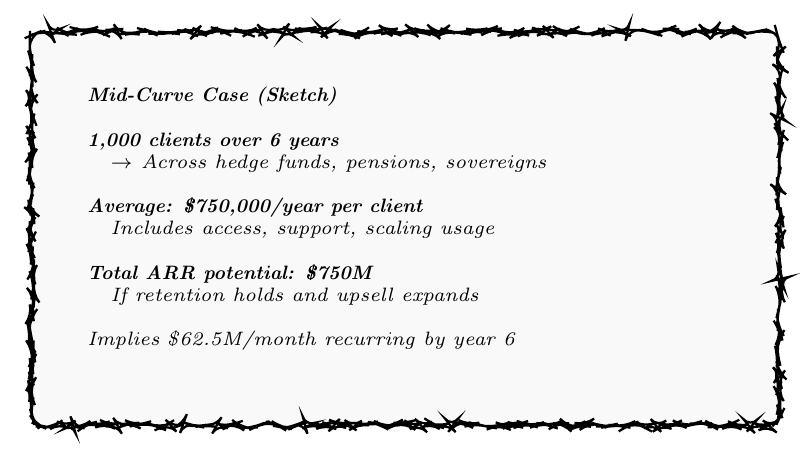
\begin{tikzpicture}[
      font=\footnotesize,
      fuzz/.style={draw=black, thick, rounded corners, fill=gray!5, decorate, decoration={random steps, segment length=2pt, amplitude=1pt}},
      txt/.style={align=left, font=\scriptsize\itshape},
    ]
  
    % Napkin box
    \node[fuzz, minimum width=9.5cm, minimum height=5cm, anchor=north west] (napkin) at (0,0) {};
  
    % Content inside
    \node[txt, anchor=north west] at ([xshift=0.6cm, yshift=-0.6cm]napkin.north west) {
      \textbf{Mid-Curve Case (Sketch)} \\
      \\
      \textbf{1{,}000 clients over 6 years} \\
      \quad $\rightarrow$ Across hedge funds, pensions, sovereigns \\
      \\
      \textbf{Average: \$750{,}000/year per client} \\
      \quad Includes access, support, scaling usage \\
      \\
      \textbf{Total ARR potential: \$750M} \\
      \quad If retention holds and upsell expands \\
      \\
      \textit{Implies \$62.5M/month recurring by year 6}
    };
  
    \end{tikzpicture}
    \caption{Napkin Sketch: Mid-curve projection for enterprise ML infrastructure revenue.}
\end{figure}

\medskip

\begin{TechnicalSidebar}{What is ARR and Why Does It Matter?}

  \textbf{ARR}, or \textit{Annual Recurring Revenue}, is a core metric for evaluating the health and scalability of 
  a subscription-based business.  
  It answers one question: \textbf{If we changed nothing, how much revenue would we make next year?}
  
  \medskip
  
  Unlike one-time sales or services, ARR assumes continuity — customers staying onboard, renewals flowing in, and 
  contracts holding steady.  
  This makes it a preferred benchmark for investors, especially in enterprise SaaS, infrastructure, and 
  fintech platforms.
  
  \medskip
  
  \textbf{Why do investors care?}

  \medskip
  
  \begin{itemize}
    \item \textbf{Predictability:} ARR provides visibility into future cash flows.
    \item \textbf{Scalability:} High ARR growth often implies network effects or strong product-market fit.
    \item \textbf{Valuation:} Many high-growth companies are valued as a multiple of ARR, not EBITDA or profit.
  \end{itemize}
  
  \medskip
  
  \textbf{Here's a back-of-envelope example:}  
  1,000 clients paying \$750K/year = \$750 million ARR.  
  If we assume a 10x revenue multiple then we get a \$7.5B potential valuation.
  
  \medskip
  
  \textit{In short: ARR is more than just a finance number.}  
  It’s the story of future certainty, told in dollars per year.
  
\end{TechnicalSidebar}

\medskip

They had moved to the bar by then. The dinner plates were cleared. Hart’s jacket was off, his sleeves pushed up, and the 
lights had dimmed just enough to signal that the crowd was thinning, but not enough to end the night.

A jazz trio murmured in the corner. Ice clinked in lowball glasses. David swirled his scotch, letting the silence stretch 
before continuing.

\medskip

``And that’s just the base stack,'' Morales said, gesturing with his glass.  
``We can spin out modules like data engines, stress frameworks, and volatility overlays.  
Each one’s a license vector. Or an acquisition target.''

Hart nodded slowly, scribbling something onto a cocktail napkin.

``At a 10x revenue multiple, that’s a \$7.5 billion ceiling.''

He looked up. ``But that’s not the point.  
The point is to scale past everyone’s comfort zone — fast enough that no one catches up.''

David leaned back, watching the amber catch in the bar light.

``You won’t get there by pitching dashboards,'' he said.  
``You need belief. You need momentum. And you need a fear of missing out.''

Hart raised his glass, smiling. ``Exactly. Blitz the market. Control the myth.''

David tapped his glass gently against Hart’s. ``You won’t get there without narrative control.''

``That’s why we’re building the narrative ourselves,'' Hart said, and drank.


\medskip

\begin{HistoricalSidebar}{The Blitzscaling Playbook: Growth First, Friction Later}

  The term \textbf{blitzscaling} was popularized by LinkedIn founder Reid Hoffman and entrepreneur Chris Yeh in their 
  2018 book of the same name.  
  It describes the strategy of prioritizing \textbf{rapid scaling over efficiency}: deliberately accepting chaos, instability, 
  and short-term loss in pursuit of long-term dominance.
  
  \medskip
  
  \textbf{The idea?} In winner-take-most markets (especially network-based or tech-driven), the biggest risk isn’t 
  inefficiency. The biggest risk is irrelevance.  

  \medskip

  The first company to reach critical scale locks in network effects, captures users, and scares off late-stage capital 
  for competitors.
  
  \medskip
  
  These are the core blitzscaling tactics:

  \medskip
  
  \begin{itemize}
    \item \textbf{Ignore traditional management advice.} Scale even when systems aren’t ready.
    \item \textbf{Outspend competitors.} Win land grabs before profit matters.
    \item \textbf{Hire ahead of revenue.} Prioritize coverage and speed over org clarity.
    \item \textbf{Fundraise fast and frequently.} Capital becomes both fuel and moat.
  \end{itemize}
  
  \medskip
  
  
  Consider the case of AirBnB. 

  \medskip
  
  In 2011–2013, AirBnB was losing money in most markets. Its customer service operations were 
  overwhelmed, and regulators were circling. However, its leadership doubled down on blitzscaling:
  
  \begin{itemize}
    \item Rapid geographic expansion to dozens of cities per quarter.
    \item Aggressive marketing with subsidized travel, and referral programs.
    \item Growing headcount, scaling trust \& safety, increasing support, and engineering all at once.
  \end{itemize}
  
  \medskip
  
  The result?

  \medskip
  
  \begin{itemize}
    \item In 2011: Airbnb was valued at \$1B.
    \item By 2014: \$10B.
    \item And by IPO in 2020: over \$100B.
  \end{itemize}
  
  \medskip
  
  Blitzscaling worked, but it wasn't without cost:  
  Legal battles, housing backlash, employee burnout, and early investor dilution were all part of the path.
  
  \medskip
  
  \textbf{The takeaway?}  
  Blitzscaling is a bet that \textit{dominance now} is worth \textit{disarray today}.  
  It’s not for every company. However, in capital-rich, timing-sensitive markets, it can be the difference between first place 
  and forgotten.
  
\end{HistoricalSidebar}


\subsection*{Editor Questions for ``The Pitch Behind the Pitch''}

To get meaningful and diverse feedback, I designed these questions to go beyond surface-level edits.
I need you to reflect not just on technical clarity or style, but on emotional resonance, character
believability, narrative structure, pacing, and thematic depth. You don’t need to answer every question.
Please focus on the ones that speak to your experience as a reader. The goal is not to fix the scene,
but to understand how it lands, where it connects, and where it might quietly miss.

\subsubsection{Narrative \& Structure}

\begin{itemize}
\item Did the three-part arc — the pitch, the calculus, and the napkin math — feel cohesive and well-structured?
\item Did the pacing work across scenes, or did any part feel too slow or too dense?
\item Was there a clear sense of escalation or momentum across the conversations?
\item Would breaking it into more chapters or scene breaks help readability or impact?
\end{itemize}

\subsubsection{Emotional Resonance}

\begin{itemize}
\item How did this sequence make you feel? Excited? Intrigued? Disoriented?
\item Were there moments where you felt emotionally connected to David — or distanced?
\item Did the mood and setting (e.g., scotch, jazz, marble tables) contribute meaningfully to the tone?
\end{itemize}

\subsubsection{Character Insight}

\begin{itemize}
\item Did Hart feel like a compelling presence — someone with depth, or mostly a rhetorical device?
\item Did David feel passive or active in the negotiation? Was that satisfying?
\item How well did Morales' voice stand apart from Hart’s? Could you distinguish the characters clearly?
\end{itemize}

\subsubsection{Thematic Cohesion}

\begin{itemize}
\item What themes did you take away from this scene? Control, access, valuation, myth?
\item Did the recurring metaphors (gateways, keycards, time arbitrage) feel earned or overused?
\item Do the technical details enhance or dilute the deeper message?
\end{itemize}

\subsubsection{Technical \& Expository Balance}

\begin{itemize}
\item Did the technical sidebars feel integrated with the narrative or too standalone?
\item Was there any part of the explanation (e.g., synthetic credit, ARR) that dragged or confused?
\item Were the Fermi estimates and market sizing believable and satisfying as a reader?
\end{itemize}

\subsubsection{Style \& Voice}

\begin{itemize}
\item Did the prose feel immersive, too ornate, or just right for this genre and tone?
\item Was there a line or image that stood out (positively or negatively)?
\item Did the dialogue feel stylized in a way that served the tone, or did it ever feel unnatural?
\end{itemize}

\subsubsection{Deeper Testing}

\begin{itemize}
\item If the historical and technical sidebars were removed, how much narrative weight would be lost?
\item If this were the only chapter you read, what would you assume the book is about?
\item What kind of reader is this written for? Did you feel included, excluded, or challenged?
\end{itemize}





\section{The Term Sheet Conversation}

\subsection{Three Men, and No Witnesses}
The room wasn’t just quiet. It was engineered that way.
Leather booths, mahogany walls, and a chandelier that gave off more shadow than light.

No laptops. No notepads. Just scotch, espresso, and the shared understanding that there was 
no need for an NDA.

Penn sat between them with his legs crossed.
He wasn’t counsel tonight; at least, not officially.
But Hart had worked with him before, and Morales knew his reputation:
Former general counsel at Sovereign Equities, now freelancing in the grey zones as part fixer, and part 
forensic mapmaker.
He didn’t take sides. He kept the paper clean, the edges sharp, and the timeline short.
If a deal was going to break later, it wouldn’t be because the documents were sloppy.

Hart leaned back with his jacket open and a half-smile behind the rim of his glass.
Morales stayed straighter, arms on the table, watching Penn turn each page like he was parsing a hidden code.

``You both know how this works,'' Penn said finally, ready to create the draft down without drama. 

Three glasses clinked softly.
The conversation began.

\medskip

\begin{TechnicalSidebar}{Term Sheets — The Architecture of Agreement}

  A \textbf{term sheet} is not a contract. It’s a prelude — a non-binding agreement that outlines the essential terms 
  and structure of a potential deal. Think of it as the architectural sketch before the blueprints are drafted.
  
  \medskip
  
  In venture and joint venture contexts, term sheets cover the core pillars of control and value:

  \medskip
  
  \begin{itemize}
    \item \textbf{Valuation:} Pre-money vs. post-money estimates define how much the company is “worth” — on paper — 
    before and after new investment enters.
    \item \textbf{Equity Split:} Who owns how much, often expressed in authorized shares or percentage ownership.
    \item \textbf{Governance Rights:} Who gets board seats, voting power, or vetoes over key decisions.
    \item \textbf{Capital Commitments:} How much money is going in, from whom, and on what terms (equity, debt, SAFE, etc.).
    \item \textbf{IP Ownership:} Who controls patents, algorithms, or trade secrets — especially important in tech or 
    biotech ventures.
    \item \textbf{Exit Preferences:} Clauses outlining what happens in IPO, acquisition, or liquidation scenarios.
  \end{itemize}
  
  \medskip
  
  While non-binding in most clauses, for final agreements, a term sheet sets the tone, and precedent. Concessions made 
  here often calcify into structure. That’s why seasoned negotiators use term sheets not just to define economics, but to 
  test boundaries, establish leverage, and signal priorities.
  
  \medskip
  
  The term sheet isn’t just a document. It’s a litmus test of trust. Penn’s role isn’t to sell 
  or oppose the deal, but to ensure no one can later say: ``I didn’t know what I was agreeing to.''
  
\end{TechnicalSidebar}

\medskip

\subsection{The Offer}

The restaurant had nearly emptied. Only a few tables remained, their patrons deep in wine or conversation too serious to pause. 
Outside, the streetlights haloed in the mist. Inside, the air was low and warm, thick with the last hour’s bourbon and ambition.

They were still at their corner table. The waiter had stopped checking in.

Hart leaned forward, resting his elbows on the linen-draped table, his voice even.

``We don’t need to overcomplicate this.''

He drew a slow line on the edge of his napkin with a thumbnail, then met David’s gaze.

``Aurora brings the code.''

He tapped the table once.

``Centauri brings the clients.''

Another pause.

``Fifty-fifty on profits. Post cost recovery. No cap table entanglement.''

He let it hang: simple, clean, and heavy with implication.

\medskip

\begin{TechnicalSidebar}{Why “No Cap Table Entanglement” Matters}

  In startup finance, the \textbf{cap table} (capitalization table) is the definitive ledger of ownership:  
  who owns what percentage, how much dilution has occurred, and what each shareholder is entitled to in exit scenarios.
  
  \medskip
  
  Cap tables govern more than equity. They govern \textbf{control}.  
  Any changes — even minority stakes — can trigger rights to board seats, voting power, information access, or liquidation preferences.  
  They also signal to investors and regulators that an entity is \textbf{financially intertwined}, which can raise red flags.
  
  \medskip
  
  \textbf{Why avoid cap table entanglement here?}

  \medskip
  
  \begin{itemize}
    \item \textbf{Regulatory distance:} Centauri works with sensitive government clients. Formal equity in Aurora 
    might subject Centauri to scrutiny for co-owning a black-box algorithm.
    
    \item \textbf{Liability firewall:} Keeping Aurora off the cap table limits legal exposure. If Aurora’s code 
    causes harm or compliance failure, Centauri can claim it was a vendor, not a subsidiary.
    
    \item \textbf{Clean optics:} No shared ownership means no complex disclosure requirements. It helps both 
    companies maintain a narrative of independence — useful for audits, investors, and press.
  
    \item \textbf{Operational speed:} With no equity entanglement, they avoid drawn-out negotiations over 
    valuation, vesting, or board control. Deals move faster when nobody’s marrying the other’s risk.
  
  \end{itemize}

  \medskip
  
  In short, ``no cap table entanglement'' isn’t about trust. It’s about insulation.  
  Hart is structuring a joint venture that behaves like a partnership — but leaves no paper trail of shared ownership.
  
\end{TechnicalSidebar}

\medskip

\subsection{The Legal Architecture}

The scotch had thinned in their glasses, condensation gathering at the base like unclaimed risk. David leaned forward, 
elbows brushing the edge of the marble, his voice low and dry. ``Sounds tidy. Until someone loses a contract or a 
courtroom summons.''

Hart didn’t miss a beat. He tipped his glass slightly, not drinking, just thinking. “That’s why we house it in a 
Delaware LLC,” he said, as if this was already settled doctrine. “Joint venture. Clean lines. Limited liability.”

He reached for a pen, drew a rough box on the corner of a folded placemat, then split it in two. “Each party is 
protected from the other’s operational mess,” he continued, drawing a clean line down the middle. “Micheal 
handles enterprise and government relationships.”

There was a pause. The low hum of ambient jazz filled the space between the words.

“David,” Hart finished, tapping his side of the box, “stays buried in the stack.”

David’s eyes lingered on the napkin, then flicked up. Outside, a passing truck washed a blur of red light across 
the bar window. Inside, everything was still. The kind of stillness you only get when both parties understand 
the real terms are unspoken — and that the real protection isn’t in the paperwork, but in the distance it creates.

\medskip

\begin{TechnicalSidebar}{Legal Sandboxing, Blame Containment, and Strategic Clarity}

  A joint venture housed in a \textbf{Delaware LLC} isn’t just convenient. It’s a structural firewall.  
  It provides \textbf{governance flexibility}, \textbf{legal insulation}, and most critically: \textbf{strategic blame 
  compartmentalization}.
  
  \medskip
  
  \textbf{Why Delaware?}

  \medskip
  
  \begin{itemize}
    \item \textbf{Predictable Legal System:}  
    Delaware’s Court of Chancery is a dedicated business court with over two centuries of case law. Corporate actors 
    know what to expect — crucial in ambiguous or high-stakes ventures.
  
    \item \textbf{Governance by Contract:}  
    Unlike other states, Delaware LLCs let parties write their own internal rulebook: covering voting rights, vetoes, 
    profit splits, and control boundaries. This minimizes surprises and aligns power with exposure.
  
    \item \textbf{Anonymity and Opacity:}  
    Delaware does not require disclosure of LLC members or managers in public filings. This enables sensitive relationships 
    to exist without triggering market scrutiny or regulatory flags.
  
    \item \textbf{No State Income Tax (for out-of-state ops):}  
    If the LLC doesn’t operate physically in Delaware, it pays no state income tax there — a quiet but attractive feature 
    for lean or distributed ventures.
  
    \item \textbf{Widely Recognized Format:}  
    VCs, MNCs, and regulatory agencies are familiar with Delaware LLCs. Enforcement, arbitration, and liability 
    interpretation are all streamlined (especially in cross-border or federal contexts).
  \end{itemize}
  
  \medskip
  
  The Delaware LLC acts as a \textbf{buffer entity}:

  \medskip
  
  \begin{itemize}
    \item To a \textbf{regulator}, Centauri appears to own and operate the deployment (they’re the visible face).
    \item To a \textbf{court}, Aurora’s contribution is buried in backend infrastructure (meaning their exposure 
    is indirect, if not fully deniable).
  \end{itemize}

  \medskip
  
  This structure enables:

  \medskip
  
  \begin{itemize}
  \item \textbf{Plausible deniability for the engineers.}  
  \item \textbf{Regulatory insulation for the client-facing firm.}  
  \item \textbf{And shared upside without shared liability.}
  \end{itemize}

  \medskip
  
  It’s not just a company. It’s a liability boundary that is wrapped in Chancery-grade contract law.
  
\end{TechnicalSidebar}

\medskip

\subsection{The Intellectual Property Play}

The noise in the lounge had dipped into a murmur, just espresso cups and legal pads now. Penn spoke first, quietly but 
firmly, without looking up from his notes. “IP ownership?”

Hart didn’t hesitate. ``Aurora holds the core protocol and infrastructure rights,” he said, eyes flicking toward David. 
“Centauri gets exclusive licenses in the verticals that matter: defense, health data, anything cross-border.''

David, half-shaded by the corner lamp, gave a small nod, then asked the question that had been pressing at him all week. 
``And the core ML stack? My algorithms?''

``They’re trade secrets,'' Hart replied. ``Right now, buried deep. No public disclosure. But if we want institutional traction, 
that’s not enough.''

He leaned forward, elbows creasing the legal pad in front of him. ``You file just enough provisional patents to fence the 
territory. That gives us a portfolio we can price. A valuation narrative that isn’t just code, but capital.''

Penn looked up now, his brow furrowed. ``So even if we’re pre-revenue...''

Hart nodded before he could finish. ``We’re patent-rich. It’s not just protection. It’s positioning.''

\medskip

\begin{TechnicalSidebar}{Patent Portfolio Valuation: Strategic Leverage through IP Architecture}

    \textbf{Overview:}  
    Patent portfolios are not just legal shields — they are financial instruments. They allow firms to price 
    their technological advantage, justify pre-revenue valuations, and negotiate licensing leverage. Below 
    are the core valuation pillars and how each contributes to an aggregate IP-based valuation narrative.
    
    \medskip
    
    \textbf{1. Core Technology Coverage:}  
    \textit{Protects the key innovation that underpins the company’s product and revenue model.}

    \medskip

    \begin{itemize}
      \item Estimate potential market capture.
      \item Quantify how much of that market is secured by the patents.
      \item Use discounted cash flow (DCF) to approximate per-patent value.
      \item Total Contribution: Anchors the top-line IP valuation.
    \end{itemize}

    \medskip


    \textit{Analogy: Owning the engine blueprints, not just the car doors.}
    
    \medskip
    
    \textbf{2. Manufacturing \& Process Efficiency:}  
    \textit{Covers proprietary methods that lower production or operational costs.}

    \medskip
    \begin{itemize}
      \item Calculate annual cost savings due to protected processes.
      \item Apply DCF to those savings to estimate long-term benefit.
      \item Distribute value across process-related patents.
    \end{itemize}

    \medskip

    \textit{Analogy: Patents that shave dollars off every unit made.}
    
    \medskip
    
    \textbf{3. Application-Specific Expansion:}  
    \textit{Enables product line diversification and licensing into new sectors.}

    \medskip
    \begin{itemize}
      \item Forecast licensing or new adoption revenue by vertical.
      \item Value protected use-cases via DCF and strategic mapping.
    \end{itemize}

    \medskip

    \textit{Analogy: A single tool with patents that unlock new industries.}
    
    \medskip
    
    \textbf{4. Safety, Reliability, and Regulatory Edge:}  
    \textit{Reduces compliance risk and improves real-world operability.}

    \medskip
    \begin{itemize}
      \item Estimate avoided costs (recalls, delays, fines).
      \item Quantify valuation boost from regulatory clearance advantage.
    \end{itemize}

    \medskip

    \textit{Analogy: Patents that prevent billion-dollar mistakes.}
    
    \medskip
    
    \textbf{5. Emerging Innovation:}  
    \textit{Covers speculative or early-stage filings that future-proof the roadmap.}

    \medskip
    \begin{itemize}
      \item Estimate future market potential and strategic optionality.
      \item Value provisional patents based on trajectory and signal value to investors.
    \end{itemize}

    \medskip

    \textit{Analogy: Seeds for the next product line — not revenue today, but leverage tomorrow.}
    
    \medskip
    
    \textbf{6. Team \& Competitive Advantage:}  
    \textit{Valuation uplift from founder IP ownership and technical exclusivity.}

    \medskip
    \begin{itemize}
      \item Assign market premium from proprietary knowledge.
      \item Apply industry revenue multiples based on talent-IP coupling.
    \end{itemize}
    \textit{Analogy: Not just owning the patents — owning the people who wrote them.}

    \medskip
    
    
    \textbf{Strategic Outcome:}  
    A well-scoped patent portfolio transforms intellectual capital into financial leverage — enabling 
    pre-revenue companies to justify valuation, attract institutional capital, and block competitors 
    without a single dollar of revenue.
    
\end{TechnicalSidebar}

\medskip

He glanced at David again, making sure the next part landed. ``We don’t sell source code. We sell 
defensible moats. That’s what funds benchmark. That’s what strategics acquire.''

David’s voice was quieter now, but sharper. ``And I stay first inventor?''

``Of course,'' Hart said, with the easy confidence of someone who had already papered a dozen cap 
tables. ``We’ll frame it as corporate prestige — first author status, conference decks, citation 
credits.''

He smiled, not quite warmly. ``You get the podium. We get the IP lock-in.''

\medskip

\begin{HistoricalSidebar}{Moats, Markets, and Musk: A Tale of Two Philosophies}

  \textbf{Warren Buffett} famously coined the term \textbf{“economic moat”} to describe a sustainable competitive advantage — 
  something that protects a company’s long-term profitability from rivals. For Buffett, moats came in many forms: 
  brand loyalty, regulatory barriers, pricing power, and network effects.  
  
  \medskip
  
  His thesis was simple: if a business has a wide enough moat, it can withstand market attacks and continue compounding value. 
  Coca-Cola, American Express, and Geico were all Buffett favorites not because they were flashy, but because they were 
  \textbf{resilient}.  
  
  \medskip
  
  Then along came \textbf{Elon Musk}.  
  
  \medskip
  
  In a 2018 earnings call, when asked about Tesla’s competitive moat, Musk scoffed:
  
  \begin{quote}
  Moats are lame. They’re like nice in a sort of quaint, vestigial way. If your only defense against invading armies 
  is a moat, you will not last long. What matters is the pace of innovation.
  \end{quote}
  
  \medskip
  
  Instead of defending territory, Musk advocated for outpacing rivals through relentless iteration.  
  He viewed moats as signs of stagnation — the tools of incumbents, not disruptors.
  
  \medskip
  
  The clash reveals a deeper split in philosophy:  

  \medskip
  
  \begin{itemize}
    \item Buffett believes markets reward defensibility.
    \item Musk believes markets reward velocity.
  \end{itemize}
  
  \medskip
  
  And in that contrast lies a dilemma for modern startups:  
  \textit{Build a castle, or build a rocket?}  

  \medskip
  
  Moats attract capital. Speed wins headlines.  
  Smart founders — like Hart — try to sell both.
  
\end{HistoricalSidebar}

\medskip

\subsection{The Division of Risk}

The table was cluttered with half-drained espresso cups and a napkin collage of diagrams, margins scribbled with 
arrows and acronyms. Rain slid down the window in quiet rivulets, muting the late-night city beyond.

Morales leaned back, arms crossed. “So we’re the backend, and you’re the storefront,” he said, voice low. “But 
if something breaks, you expect us to take the fall?”

Hart met his gaze evenly. “Not just the fall. The heat,” he said. “Our liability stops at the interface. We own 
the relationship. You define the implementation.”

Morales glanced at Penn, then back at Hart. “So we take the risk?”

Hart didn’t blink. “You also take the upside.”

He paused just long enough to imply a shift in tone, then added, “Look, naturally you'd have veto power. 
I’m not touching your stack. My job is to sell, not to interfere. You tell me what’s real, what’s stable, 
and what’s still in flight. Then I build the story around that. You always have the right to say no. 
That’s the deal.”

David arched a brow, cautious.

“I don’t pretend to understand the tech,” Hart continued, softer now, more surgical. “That’s your world. You built it. 
You know what it can and can’t do. That’s why I handle the clients, and you handle the system.”

A long silence followed. Outside, a car passed, headlights flickering across the ceiling. David finally nodded once, 
not agreement exactly, but something close to acceptance. Or the beginning of it.

\medskip

\begin{TechnicalSidebar}{Liability Follows the Paperwork}

  In corporate law, \textbf{liability is a function of structure}.  
  Who takes the hit when something fails isn’t just a matter of causality. It’s a matter of incorporation, contracts, 
  and jurisdiction.
  
  \medskip
  
  In a \textbf{joint venture LLC}, liability can be ring-fenced. For example:

  \medskip

  \begin{itemize}
    \item If \textbf{Centauri} owns the customer contract and the branding, it's Centauri that faces legal exposure when the 
    system fails — even if the bug originated in Aurora's code.
    \item \textbf{Aurora}, by staying "behind the interface" and licensing its technology, can argue it is merely a vendor — 
    not the operator.
  \end{itemize}
  
  \medskip
  
  This design is intentional.  
  It creates a structure in which:

  \medskip

  \begin{itemize}
    \item \textbf{Regulators} see one party as accountable — the one with the deployment contract.
    \item \textbf{Courts} assess liability based on terms of use and operational control, not source code authorship.
  \end{itemize}
  
  \medskip
  
  Examples:

  \medskip

  \begin{itemize}
    \item \textbf{Apple and Foxconn:} When iPhones catch fire, Apple takes the PR hit, even though Foxconn assembled the device.
    \item \textbf{Boeing and subcontractors:} Boeing owns the jet. If a subcontractor’s software fails, Boeing still gets sued.
    \item \textbf{Google Cloud and third-party models:} If a bank misuses a third-party ML model deployed on GCP, Google can claim it's just the infrastructure — not the policy-maker.
  \end{itemize}
  
  \medskip
  
  \textbf{Bottom line:}  
  Structure liability correctly, and failure becomes survivable.  
  Misplace it, and the wrong engineer ends up testifying before Congress.
  
\end{TechnicalSidebar}

\medskip

\subsection{The Arrangement}

The hotel bar had mostly emptied. The few remaining guests were either winding down or too deep in conversation to 
care who overheard. Hart’s glass was half-full, his tone anything but.

“Private equity?” he said, grinning as he leaned back against the leather banquette. “That’s small beans. They think 
in three-, five-, maybe ten-year returns.” He swirled his drink. “I sell to clients who don’t exist until the 
third NDA.”

He leaned forward now, lowering his voice like he was reciting doctrine. “You’re thinking in rounds. 
I’m thinking in regimes.”

Morales raised an eyebrow, and Hart pressed on, tapping a finger lightly against the table. “You know code. 
You know scale. But I know how to package this for a sovereign fund with no official website. For a ministry whose name 
changes every fiscal quarter.”

The napkin between them was already covered in boxes, arrows, and marginalia. Hart pointed to a blank space. “You 
write the protocol. I’ll get it in the hands of someone who doesn’t shake hands. Just gives nods.”

“And governance?” Morales asked, tone cautious.

Hart gave a practiced shrug. “Joint oversight. You get roadmap visibility and veto power on enterprise deployments. 
We retain control over base-layer changes. We’re not getting dragged into client-specific rewrites every time a 
lame government employee\footnote{
It’s an open secret in finance and tech: many insiders dismiss government regulators as \emph{``lame government 
employees''}—slow-moving, risk-averse, and allergic to innovation. The dynamic is perhaps best embodied by Elon Musk’s 
famously combative relationship with the SEC. After being fined for his “funding secured” tweet about taking Tesla 
private, Musk referred to the agency as the \emph{“Shortseller Enrichment Commission”} and joked on \emph{60 
Minutes} that he had “no respect” for them. The subtext wasn’t subtle: in the eyes of high-velocity capital, 
regulation is often treated as an obstacle to be gamed, not a principle to be honored.
}
panics about regulation.”

Penn had been quiet, flipping a coaster between her fingers, but now she looked up. “Revenue waterfall?”

Hart didn’t hesitate. “Topline gets cleared for costs. Then split fifty-fifty. We’ll handle infrastructure spend. You 
handle channel activation. We’ll memo it clean. However,” he held up a finger, “the key principle is: \textit{
  If you don't build then we don’t sell}”

Morales cracked a tired grin. “A joint venture,” he said, “or just plausible deniability in a trench coat?”


\medskip

\begin{TechnicalSidebar}{Strategic Insulation via Joint Ventures}

  This structure — Centauri fronting the client relationships while Aurora provides the core technical stack — is a 
  textbook example of a joint venture built for \textbf{strategic insulation}. Each party contributes value, but the 
  legal architecture is designed to contain fallout.
  
  \medskip
  
  Here’s how it works:

  \medskip
  
  \begin{itemize}
    \item \textbf{Delaware LLC structure} ensures pass-through tax treatment and contractual flexibility.
    \item \textbf{Exclusive vertical licenses} give Centauri sales rights in high-margin sectors (defense, health) without 
    requiring cap table involvement.
    \item \textbf{Ownership vs. Liability Split:}
      \begin{itemize}
        \item Aurora owns the code (and patents), so it becomes the \textit{technical authority}.
        \item Centauri owns the client narrative, so it becomes the \textit{political authority}.
      \end{itemize}
    \item \textbf{Cost Recovery + Profit Split} makes the economics look fair, while strategically keeping Aurora dependent 
    on Centauri’s access.
    \item \textbf{Clause: “We don’t sell. You don’t build.”} ensures role separation — and liability separation — in case 
    of failure.
  \end{itemize}
  
  \medskip
  
  In legal terms, this is a \textbf{risk-pooling mechanism}. In practical terms, it’s a way to let Aurora take the engineering 
  risk while Centauri harvests the reputational upside.
  
  \medskip
  
  David may think he’s a founder brokering a partnership.

  \medskip
  
  But on paper?

  \medskip
  
  \textbf{He’s an unwitting contractor, fronting liability for someone else’s empire.}
  
\end{TechnicalSidebar}


\medskip

\subsection{The Cap Table Discussion}

The waiter dropped off a fresh pot of coffee. Penn pushed aside her empty espresso and flipped to the second page of the 
term sheet, the paper already creased from too many folds.

``What’s the par value?'' she asked, eyes scanning the cap table clause.

Morales didn’t look up. ``One cent a share. We authorize ten million. Keeps the math clean, and gives us room for 
dilution later.''

Hart leaned in, tapping his pen against the edge of a coaster. ``And we split fifty-fifty?''

``Five million shares each,'' Morales confirmed with a nod. ``We each put in \$100,000 to match. It keeps the equity 
clean and symmetrical.''

Penn underlined a section with the edge of her nail, then glanced up. ``And what about board structure?''

Morales raised an eyebrow. ``Simple. Two seats: one for Aurora, one for Centauri. We deadlock, we defer.''

Hart gave a faint grin. ``Let’s just not deadlock then.''

\begin{TechnicalSidebar}{Par Value And Why It Matters}

  \textbf{Par value} is the nominal or “face” value of a company’s stock as stated in its charter. Historically, it 
  represented the minimum price at which shares could be issued: a protection against companies selling stock below 
  worth. Today, especially in startup contexts, par value is largely symbolic --— often set at \$0.01 or even 
  \$0.0001 —-- but it still plays several important roles:
  
  \medskip

  \begin{itemize}
    \item \textbf{1. Legal and Tax Anchor:}  
    Par value determines the company’s initial legal capital: the amount that cannot be returned to shareholders 
    in the event of insolvency. If a company issues 10 million shares at \$0.01 par value, its legal capital is 
    \$100,000. This becomes relevant in bankruptcy or during shareholder litigation.
    
    \item \textbf{2. Founders’ Contribution Benchmark:}  
    Setting a non-zero par value (e.g., \$0.01) ensures founders actually pay something for their shares. In this 
    case, both founders contribute \$100,000 for 5 million shares each which aligns equity with skin in the game 
    and reducing IRS scrutiny of “free” founder stock.
    
    \item \textbf{3. Clean Cap Table and Signaling:}  
    By keeping par value low, companies retain flexibility to issue large numbers of shares to future investors, 
    advisors, or employees without creating accounting headaches. It also makes the share count feel larger, and  
    it's useful for signaling scale or structuring option pools.
    
    \item \textbf{4. Downstream Compliance:}  
    During diligence or fundraising, VCs, auditors, and regulators often review how the company handled par value 
    and capital contributions. A sloppy or arbitrary setup can raise questions about governance maturity.
  \end{itemize}
  
  \medskip
  
  \textit{In short:} Par value is a humble line on a charter. However, it shapes the earliest story a company tells 
  about who owns what, who paid what, and what’s legally at stake.
  
\end{TechnicalSidebar}

\subsection{The Valuation Play}

The overhead lights buzzed softly as the three of them sat around the polished walnut table, the term sheet now marked with coffee rings and margin notes. The air was quiet, but not still — it was the silence of people calculating.

Penn set down her pen and looked up. ``And the valuation?''

Morales leaned back slightly. ``Under a million post-money. Low on paper — for now. But once the patents clear, we reprice.''

Hart tapped his index finger on the table, three times in rhythm. ``Three filings, minimum: synthetic hedging stability, 
volatility symmetry, and stress-optimized reinforcement. If we license those into the venture structure, we’re looking at 
thirty to fifty million in defensible value, pre-revenue.''

Penn gave a low whistle, then scanned the clause again. ``So the par value gives you maximum control at minimum cost. And 
the IP does the heavy lifting later?''

``Exactly,'' Hart said. ``Value isn’t just built. It’s signaled.''

Morales added, ``And nothing signals harder than three patents wrapped in a Delaware corp with a clean cap table.''

Hart raised his glass. ``To value created. And to value believed.''

\medskip

\begin{TechnicalSidebar}{Patent Portfolio Valuation}

  In early-stage ventures, especially in tech and biotech, intellectual property (IP) isn’t just a protective shield. 
  It’s a valuation engine. A well-positioned patent portfolio can drive funding, justify premiums, and shift power 
  dynamics long before revenue arrives.
  
  \medskip

  \begin{itemize}
  
    \item \textbf{1. Patents as Non-Dilutive Leverage:}  
    Filing patents allows a founder to inject value into the cap table without raising capital or giving up equity. 
    The patent becomes an asset: one that can be licensed, pledged, or used to anchor valuation.
    
    \item \textbf{2. Pre-Revenue Valuation Boost:}  
    Investors may assign \$10–\$20 million in valuation uplift \textit{per defensible patent}. This is especially true 
    if the filings target high-margin verticals (e.g., defense, health, or finance) or enable technical exclusivity 
    in core system components.  In this context, three filings can justify a \$30–\$50 million post-money 
    valuation (even without customers).
    
    \item \textbf{3. IP as Signaling Weapon:}  
    More than protection, patents are a narrative device. Provisional filings create PR events. Issued patents 
    validate technical credibility. And exclusivity clauses --— when licensed into the venture --— transform IP 
    into competitive moats investors can underwrite.
    
    \item \textbf{4. Delaware Structure + Clean Cap Table = Signal Amplifier:}  
    When housed in a Delaware C-corp with clear equity splits and no messy SAFEs or option overhangs, patents 
    send a strong message: this company knows how to tell a story investors can believe in.

  \end{itemize}

  \medskip
  
  \textit{Bottom line:}  
  In the startup economy, patents aren’t just protection. They’re pre-revenue currency.  
  And the stronger the story behind the filing, the higher the multiplier on belief.
  
\end{TechnicalSidebar}






\section{After the Ink Dried}

\subsection{Tell Me Something Real}

The hotel bar was a study in controlled elegance: dark wood, low ceilings, and jazz that didn’t 
quite reach the back corner booth.
That’s where Hart sat, alone, sketching on a napkin with the deliberate calm of a man who already knew 
the ending.

David spotted him first.
He and Michael slid into the booth opposite, shrugging off their coats as the server brought over the 
first round without being asked.

“Tell me something real,” he said, tone casual but angled. “How’d you end up building Centauri?”

David glanced down at the glass, swirling the ice before answering.

“Honestly? I got tired of being someone else’s tail risk. Started it with my wife. She’s an analyst. 
Or was. Stepped back when we had the kids. Said raising them was harder than any corporate job.”

Hart raised his glass in a silent toast. “She sounds like the real founder.”

David laughed. “Depends on which toddler you ask.”

“How many?” Hart asked, not just to ask.

“Two. Five and three. The older one already asks what I ‘do’ all day.”

Hart nodded slowly, watching the way David’s expression shifted when he said it.
“Give it time. One day they’ll say you ‘tell people what to do and take credit for their work.’”

They clinked glasses again, the crystal tap echoing like punctuation. Behind them, the jazz slowed — 
brushes on snare, bass walking quietly beneath the room’s conversations.

\medskip

\begin{PsychologicalSidebar}{The Thin Line Between Help and Grooming}

  Psychologists use the term \textbf{grooming} to describe the process by which a more powerful actor builds trust, 
  dependency, and emotional leverage over a target—incrementally lowering their resistance to boundary violations.

  \medskip
  
  While often discussed in interpersonal or criminal contexts, the same psychological mechanisms can surface in 
  professional and institutional settings.

  \medskip
  
  At its core, grooming is a strategy of \textbf{gradual normalization}:  

  \begin{itemize}
    \item Each “favor” feels like mentorship.  
    \item Each private invitation feels like inclusion.  
    \item Each off-the-record conversation feels like trust.
  \end{itemize}

  \medskip
  
  But beneath the veneer of help lies a quiet asymmetry. The powerful actor controls access, opportunity, and escalation. 
  The recipient is positioned to feel indebted, grateful, increasingly reluctant to say no.

  \medskip
  
  In Centauri’s partnership with Aurora, the grooming wasn’t sexual or criminal—it was structural. Every dinner, every 
  introduction, every off-paper meeting created a subtle but compounding sense of \emph{obligation}.
  
  \begin{quote}
  Grooming is effective not because it overtly coerces,  but because it makes resistance feel like betrayal.
  \end{quote}
  
  The psychological danger is that the line between help and manipulation isn’t marked by intent—it’s marked by 
  \textbf{power asymmetry and conditionality}.  When help comes bundled with escalating asks, unstated expectations, 
  and deferred reciprocation, it stops being help.  It becomes preparation.
  
\end{PsychologicalSidebar}

\medskip

\subsection*{Editor Questions for ``Tell Me Something Real''}

This scene is deliberately quiet — a moment of conversational disarmament that teeters between genuine connection and strategic grooming.

These questions are meant to probe the emotional resonance, psychological layering, and implicit power dynamics.
You're not just being asked whether the scene works — but whether it seduces, disorients, or unsettles you in hindsight.

\subsubsection{Narrative \& Structure}

\begin{itemize}
\item Did this quieter, more intimate scene feel like a necessary emotional pause — or a narrative detour?
\item Was the shift in energy (from “The Catch” to this more subdued moment) effective in building tension through contrast?
\item Did the personal nature of David’s story feel earned, or too conveniently vulnerable?
\item Did the dialogue progress in a way that deepened the relational dynamic, or did it feel more expositional?
\end{itemize}

\subsubsection{Tone \& Atmosphere}

\begin{itemize}
\item How would you describe the emotional tone of the bar scene in one word?
\item Did the tone feel intimate, manipulative, or something in between?
\item Did the setting — jazz, low light, napkin sketches — contribute to the mood, or feel like stylized background?
\item Was there a sense of dramatic irony, i.e. did you feel Hart was disarming David while also studying him?
\end{itemize}

\subsubsection{Character Insight}

\begin{itemize}
\item Did you gain new insight into David in this scene? Did he feel more human, more naïve, more compromised?
\item What did you make of Hart’s role here — was he bonding, manipulating, grooming, or simply listening?
\item Did the line “She sounds like the real founder” shift your perception of Hart’s intentions?
\item Was Michael’s silence in this scene meaningful, or did he disappear narratively?
\end{itemize}

\subsubsection{Power \& Trust}

\begin{itemize}
\item Did the scene reinforce or challenge your understanding of who holds power in this relationship?
\item Did you sense that Hart was steering the conversation toward future leverage — or was it genuinely collegial?
\item Was the toast, the laughter, the unspoken camaraderie comforting or foreboding?
\item Did the exchange feel symmetrical in emotional exposure — or did Hart maintain control by revealing little?
\end{itemize}

\subsubsection{Psychological Resonance}

\begin{itemize}
\item Did the psychological sidebar on grooming alter or deepen your reading of this scene?
\item Were there moments in the dialogue where “mentorship” felt like preparation or testing?
\item Did you feel the emotional boundaries in this scene were blurred intentionally — by one or both parties?
\item If you read this scene again after reading the sidebar, did it reframe your understanding of what just happened?
\end{itemize}

\subsubsection{Craft \& Detail}

\begin{itemize}
\item Did the imagery (glass swirling, crystal clink, napkin sketching) work symbolically or feel ornamental?
\item Was there a particular phrase or moment that lingered — positively or uncomfortably?
\item Did the jazz and bar setting feel immersive — or like a trope?
\item Was the rhythm of the dialogue effective in building emotional texture and unspoken tension?
\end{itemize}

\subsubsection{Deeper Testing}

\begin{itemize}
\item If this scene were the only one you read from the story, what would you think the genre or larger theme was?
\item What would happen to the scene’s power if the sidebar on grooming were removed?
\item What would David’s wife think if she overheard this conversation?
\item What is Hart not saying — and did that silence have weight?
\end{itemize}


\subsection{Seduction by Self-Image}

“So,” Hart said, letting the silence hang just long enough, “is she the kind who reads your 
emails... or the kind who pretends not to?”

David smirked. “Neither. She ignores them completely. Says work is my sandbox. Not hers.”

“That’s rare,” Hart said, sipping his whiskey. “Most co-founders either burn out or blur the 
line. Sounds like you two still have a line.”

“We try,” David said.

“And when you don’t?”

“We fight. Then we remember we’re tired. Then we order Thai.”

Hart laughed, but only with his mouth. His eyes stayed steady. “So... domestic diplomacy.”

David shrugged. “Something like that.”

Hart traced a circle on the napkin with the side of his finger. “How do you decompress?”

“Work out. Sometimes bourbon. Mostly I just delay the crash.”

“Control’s overrated,” Hart said, tipping his glass. “Leverage is where the fun is.”

David raised an eyebrow. “You make that sound like a kink.”

Hart smiled. “Only if you’re doing it right.”

David shook his head, amused. “You always talk like that — in metaphors and maxims. Don’t 
you ever just say what you mean?”

“I do,” Hart said. “I just never say it first.”

David laughed. “That feels like something you stole from a poker manual.”

“I prefer field notes from the boardroom,” Hart said. “Same bluff, higher stakes.”

David swirled the mezcal in his glass. “So what’s this, then? A test?”

Hart leaned in slightly. “No. A calibration.”

“Of what?”

“Your equilibrium. Your tells. What you flinch at. What you dodge. What you overcompensate to defend.”

David chuckled, but something in his posture tightened. “You always profile people over drinks?”

“Only the interesting ones,” Hart said. “The rest get email follow-ups.”

“And me?”

Hart tapped the napkin, now marked with a faint spiral of condensation. “You’re worth ink.”

David stared at the napkin, then back at Hart. “Careful. Flattery’s expensive around here.”

“Only if you believe it,” Hart said. “I trade in identity, not compliments.”

David laughed again, this time with a little more edge. “You know what they call that in psychology?”

“I do,” Hart said. “But I let them name it after they lose.”

\begin{PsychologicalSidebar}{Seduction Through Identity}
Hart isn’t just making conversation. He’s reframing David’s story to highlight strength, sacrifice, and ambition.
By praising his wife and children, he signals emotional intelligence. But he also aligns himself with 
David’s self-image — a founder, a father, someone who deserves more than corporate obedience.

This leverages Cialdini’s \textbf{Consistency Principle}: once David paints himself as principled, decisive, 
and vision-driven, he becomes psychologically more likely to say yes to actions that reinforce that identity.
\end{PsychologicalSidebar}

\subsection*{Editor Questions for ``Seduction by Self-Image''}
This scene plays with identity, charisma, and psychological leverage.
It's flirtation masquerading as business, grooming disguised as banter.

These questions probe how language, pacing, and subtext guide the reader to feel complicit in the dance — even before realizing it’s a game.

\subsubsection{Tone \& Atmosphere}

\begin{itemize}
    \item Did the scene feel tense, flirtatious, manipulative, or disarming — or some blend?
    \item How would you describe the emotional temperature of this conversation? Did it shift midway?
    \item Did the dialogue rhythm (short back-and-forths, pauses, minimal exposition) work to create intimacy or uncertainty?
    \item Did Hart’s use of metaphor and deflection make him feel wise, smug, dangerous, or seductive?
\end{itemize}

\subsubsection{Character Dynamics}

\begin{itemize}
    \item What did you learn about Hart’s strategy through this conversation?
    \item Was David aware he was being profiled, or did it feel like he was complicit in the dance?
    \item Did Hart's line “I just never say it first” reveal power... or conceal something?
    \item Did David’s laugh at the end sound like confidence, discomfort, or submission to the game?
\end{itemize}

\subsubsection{Power, Flattery, \& Calibration}

\begin{itemize}
    \item When Hart says “I trade in identity, not compliments,” did that clarify or deepen the manipulation?
    \item Did the shift from casual banter to “equilibrium” and “tells” feel natural, or did it jolt the tone?
    \item Did the phrase “You’re worth ink” feel intimate, manipulative, poetic, or all three?
    \item Did the power dynamic between Hart and David feel stable — or was it oscillating?
\end{itemize}

\subsubsection{Psychological Framing}

\begin{itemize}
    \item Did the psychological sidebar help decode the scene — or did it state the obvious?
    \item Before reading the sidebar, did you sense that Hart was weaponizing identity? Or did it hit harder in hindsight?
    \item Did you feel David was being seduced by flattery — or by the idea of being understood?
    \item Does Hart’s calibration style remind you of a consultant, a predator, a therapist, or something else?
\end{itemize}

\subsubsection{Dialogue \& Style}

\begin{itemize}
    \item Was the “calibration” framing of the scene effective — or too self-conscious?
    \item Did you enjoy Hart’s poker and boardroom metaphors? Were they smooth, or risked sounding theatrical?
    \item Were there any lines that landed especially well — or others that felt too writerly?
    \item Did the napkin spiral motif work visually or symbolically?
\end{itemize}

\subsubsection{Deeper Reading}
\begin{itemize}
    \item If Hart were replaced with a woman saying the same lines, would the scene feel differently charged?
    \item If this were the first scene between Hart and David you ever read, what would you assume their relationship was?
    \item Who walks away from this conversation with more power? More information? More vulnerability?
    \item What is not being said here — and did that silence land?
\end{itemize}


\subsection{The Compliance Test}


The lights dimmed half a notch. The bar was emptying. Behind them, the bartender flipped a bar towel over his shoulder and wiped down the counter with unconscious precision.

Hart leaned in, voice quiet now, intimate.

“And when was the last time you said no... to something that felt good?”

David smiled — but it was a shield.

“That’s a dangerous question.”

Hart smiled wider. “That’s a revealing answer.”

David leaned back slightly, sipping his mezcal. “You ask that like you already know I didn’t.”

“I ask it,” Hart said, “because you’re the kind of man who mistakes momentum for inevitability.”

David raised an eyebrow. “Is that a compliment or a diagnosis?”

Hart shrugged. “Both. Useful either way.”

David set his glass down. “You always do that — phrase things just vague enough that I can't disagree without sounding insecure.”

“Would you prefer I used a slide deck?”

“I’d settle for a straight answer.”

Hart gestured at the near-empty glass between them. “I gave you one. I just used story structure instead of bullet points.”

David smirked. “And I’m supposed to what — feel seen?”

Hart’s smile tilted. “No. Just... consistent.”

David narrowed his eyes, not unkindly. “You’re playing the long game, aren’t you?”

“Aren’t we all?” Hart replied. “I’m just willing to admit it.”

A pause. Then:

“You know what your real tell is?” Hart asked.

David chuckled. “This should be good.”

“You never say yes directly,” Hart said. “You just stop saying no.”

David looked down at the napkin between them — already faintly marked from earlier sketches, damp around the edges.

“You think that means you’ve got me?”

Hart didn’t flinch. “No. I think it means you’ve already started aligning.”

“Aligning with what?”

Hart raised his glass in a silent toast. “With the version of yourself that walked into this bar already wanting to say yes.”

\begin{PsychologicalSidebar}{Commitment Bias}
Hart's seemingly harmless question about temptation creates a small but meaningful moment of disclosure.

David responds playfully, but that response is still a \textit{yes}. He didn’t push back. He participated.

That minor compliance sets the stage for deeper agreement later — a classic case of \textbf{commitment bias}: 
the tendency to remain consistent with past actions or admissions.
\end{PsychologicalSidebar}



\subsection{The Curated Reality}


By the time the last round came, the napkin had a signature.

David didn’t remember signing it.

He remembered the pacing. The rhythm. The warmth.
The moment Hart said, “We’re going to build something they’ll study.”

“You always talk like that,” David said, squinting at the napkin. “Like a historian narrating a foregone conclusion.”

Hart smiled faintly. “History is just the long-form version of good marketing.”

David shook his head. “You didn’t pitch me. You narrated me.”

“And you responded,” Hart said. “Which is more interesting than agreement.”

David picked up the napkin, studied the ink. “You ever think about just... laying out the facts?”

“I did,” Hart said. “Then I realized facts make people hesitate. Stories make them move.”

David raised an eyebrow. “So this was a story?”

Hart tapped the table once, softly. “This was a setting. The story needed a protagonist.”

“And let me guess... I’m the hero?”

“You’re the founder who walked into the bar already leaning forward,” Hart said. “I just cleared the fog.”

David gestured to the napkin. “You skipped the hard questions. Risk. Governance. Cap table mechanics.”

“I didn’t skip them,” Hart replied. “I managed the aperture. Too much light, and the subject flinches.”

David exhaled, somewhere between a laugh and a surrender. “God, you’d be terrifying with a whiteboard.”

Hart smirked. “That’s why I use napkins.”

\medskip

David leaned back, letting the glass rest in his palm. “I should feel more manipulated than I do.”

“That’s the craft,” Hart said. “Clumsy persuasion makes you feel persuaded. Good persuasion makes you feel understood.”

“Oh, so now you’re a therapist.”

Hart tilted his head. “Therapists wait for the client to speak. I build better monologues.”

“Nice. You get that from a book?”

“No,” Hart said. “From twenty years of hearing the same founders say different things and think they’re being original.”

David laughed in spite of himself. “Jesus.”

Hart didn’t break eye contact. “Look, you didn’t sign because I said something brilliant. You signed because I made the frame wide enough to fit your reflection.”


David stared at the signature again.

“You really believe they’ll study it?”

Hart took a slow sip of whiskey. “That depends.”

“On what?”

“On whether the story ends with regret... or with someone else trying to copy it.”

David nodded slowly, the weight of the night finally pressing in. “If this goes sideways...”

Hart cut in, gently. “Then we’ll control the narrative. That’s the beauty of first drafts — we get to write them.”

A long pause.

“Do you always talk people into their own decisions?”

Hart’s smile was small, but surgical. “Only the ones who already want to say yes.”

\begin{PsychologicalSidebar}{Information Control – Framing the Reality}
Hart doesn’t overwhelm David with data. He curates the lighting, tempo, and vocabulary to control perception.
This is classic information control — not through deception, but by narrowing the field of view.
By managing what is shown, what is omitted, and what is emotionally reinforced, Hart constructs a regime of truth
where David feels like the decision was his — even though every variable was engineered.
\end{PsychologicalSidebar}


\subsection{Groomed for Greatness}

Later, he’d replay that night not because he regretted it, but because he finally understood it.

Hart hadn’t just built a partnership.

He’d built a profile.
And David had been the one to hand him the raw material.

In the silence afterward — long after the bar had emptied, long after the mezcal had burned off — David 
sat in the back of the car, watching the lights blur past the window, and quietly loathed himself.

He should’ve walked away.

Right after Hart said, “Leverage is where the fun is.”
Right after Hart asked him about temptation with that grin like it was a confession booth.
Right after he sketched the entire manipulation on a napkin and passed it across the table like it was 
a contract and a dare.

He should have left. Politely. Firmly. Gratefully.
He should have said, “This was great. Let me think.”
But he didn’t.

Because somewhere under the surface — under the pride, the charm, the polish — he genuinely thought he was different.
Like Hart wouldn’t use him the same way he used the others.
Like he’d be the one to navigate the dance, not get choreographed into it.

“I told you exactly what I was doing,” Hart had said at one point, not even hiding it.
“I just never say it first.”

It was a performance, yes. But a transparent one. The kind where the trick is half the pleasure.
And David had applauded it, like an idiot.

It reminded him of a scene from Game of Thrones — a rewatch he and his wife had started after the kids 
finally began sleeping through the night.
That scene where Littlefinger tells Ned Stark not to trust him.

“I did warn you not to trust me,” Littlefinger had said, right before the knife slipped in.

Ned had nodded. He knew the reputation. Knew the man. Knew the game.

And he still trusted him.

That was Hart. That exact brand of elegant corruption.
So good he could confess the con out loud and still get the other person to lean in.
Not because he lied — but because he made the lie feel collaborative.

We’re going to build something they’ll study.
That wasn’t a pitch. That was the spell.
The kind of line that felt like a joint decision, even when it wasn’t.

And that was the truth David hated most.
Not that he’d been manipulated — but that he had agreed to it.

He wasn’t the first person Hart had profiled.
He just hated how quickly he made himself available to be read.

\begin{PsychologicalSidebar}{Weaponized Transparency}
The most effective manipulators don’t hide their tactics. They reveal them — strategically.
By confessing just enough to appear honest, they create the illusion of control, disarm skepticism,
and invite the target into a sense of co-authorship.

This is meta-manipulation: the con that doesn’t just fool you — it lets you feel clever while you’re being fooled.
It leverages a key vulnerability of high-agency individuals: the belief that they can spot the trap in time.
\end{PsychologicalSidebar}






